\section{Elektrostatik}
 

\subsection{Wichtige Formeln der Elektrostatik}
  \begin{tabular}[c]{ | p{6.5cm} | p{7cm} | p{4cm} | }
    \hline
    \textbf{Name} & \textbf{Formel} & \textbf{Einheit}\\ 
    \hline
  Dielektrizit�tskonstante
    & $\varepsilon = \varepsilon_r \varepsilon_0 = 
    \varepsilon_r 8.8542 \cdot 10^{-12} $ & $ \frac{As}{Vm}$ \\
    \hline
  Ladung
    & $Q = I t = C U$
    & $[Q] = As = C$ \\
    \hline
  Elementarladung
    & $e = 1.602 \cdot 10^{-19}$
    & C \\
    \hline
  Arbeit = Energie
    & $W_{AB} = \int \limits^b_a F(r) dr \qquad W = \int \limits^{t_1}_{t_2} p(t)
    dt$ 
    & $[W] = Ws = J; [p] = W$ \\
    \hline
  Coulombsches Gesetz (zw. 2 Q) $^{1)}$
    & $\vec{F} = \vec{E}\cdot Q \qquad F = \frac{Q_1 \cdot Q_2}{4 \pi \varepsilon
    r^2}$ & ($F>0 \rightarrow$ Abstossung) \\ \hline
  Elektrische Feldst�rke $^{2)}$
    & $\vec{E} = \frac{Q}{4\pi\varepsilon r^2} \vec{e}_r , E=\frac{Q}{4\pi\varepsilon r^2}$
    & $[E] = \frac{V}{m}$ \\
    \hline
  Potential 
    & $\varphi = \frac{W}{Q}$
    & \multirow{5}{*}{$[\varphi] = V = \frac{Ws}{As} = \frac{VAs}{As}$}
    \\ & $U_{AB} = \varphi_A - \varphi_B$ 
    & \\
    \cline{1-2}
  Potential einer Pt.-Q. 
    & $\varphi = \frac{Q_1}{4 \pi \varepsilon r}$ 
    & \\
    \cline{1-2}
  �berlagerung $>1$ Pt.-Q. $^{3)}$
    & $\varphi = \frac{1}{4 \pi \varepsilon} \sum\limits_{i=1}^n \frac{Q_i}{r_i}$
    & \\
    \cline{1-2}
  Spannung innerh. E-Feld 
    & $U_{AB} = \int\limits_A^B \vec{E}(s) d\vec{s}$
    & \\
    \hline
  Arbeit im homogenen E-Feld $^{4)}$
    & $W_{AB} = U_{AB} \cdot Q = E \cdot l_{AB} \cdot Q \cdot \cos(\alpha) $
    & $[W] = Ws = J; [p] = W$\\
    \hline
  Elektrische Flussdichte $^{5)}$
    & $\vec{D} = \varepsilon \cdot  \vec{E} = \frac{\Psi}{A} \vec{e}_r =
    \frac{Q}{A} $ & $[D] = \frac{C}{m^2} = \frac{As}{m^2}$
    \\
    & $D$ ist materialunabh�ngig 
    & \\
    \hline
  Elektrischer Fluss
    & $\Psi = \int\limits_A \vec{D} \cdot d \vec{A} \text{ od. } D \cdot dA \cdot \cos \phi$
    & $[\Psi] = As, C$ \\
    \hline
  Gauss'scher Satz der Elektrostatik 
    & $ \Psi_{Huelle} = \sum Q_{eingeschlossen} $ 
    & \\
    \hline
  Kapazit�t
    & $C = \frac{Q}{U}$
    & $[C] = F = \frac{C}{V} = \frac{As}{V}$ \\
  Kondensatoren in Serie
  	& $\frac{1}{C} = \frac{1}{C_1} + \frac{1}{C_2} + \ldots \qquad C =
  	\frac{C_1C_2}{C_1+C_2}$ & \\
  Kondensatoren parallel
    & $C = C_1 + C_2 + \ldots$
    & \\
    \hline
  Fl�chenladungsdichte
    & $\sigma = \frac{Q}{A}$
    & $ [\sigma] = \frac{C}{m^2} $\\
    \hline
  Energiedichte
      & $w=\frac{W}{V} = \frac{1}{2} \varepsilon \cdot E^2 = \frac{1}{2}D\cdot E$
      & $[w]=\frac{J}{m^3}$ \\
      \hline
  \end{tabular}


\subsection{Anmerkungen zu den Formeln}
  \textbf{1)} Gilt nur f�r Punktladungen exakt; f�r
  geladene K�rper nur wenn K�rperabmessung $\ll$ Abstand \\
  \textbf{2)} $Q > 0$: $\vec{E}$ gleiche Richtung wie $\vec{e}_r$
  $\leftrightarrow$ $Q < 0$: $\vec{E}$ entgegengesetzte Richtung wie $\vec{e}_r$t.
  Der Radius wird immer von der Kugelmitte aus genommen (d.h. an einer
  Kugeloberfl�che besteht eine Feldst�rke!)\\
  \textbf{3)} Weg AB so w�hlen, dass $\vec{E} \perp \vec{s}$ oder $\vec{E}
  \parallel \vec{s}$.\\
  \textbf{4)} Wird eine Ladung von A nach B verschoben, so h�ngt die
  aufzubringende bzw. abgeg. Energie \textit{nicht vom Verschiebungsweg}, sondern
  nur von der Potentialdifferenz $\varphi_B - \varphi_A$ ab (darum
  $\cos(\alpha)$). $\alpha$ ist der Winkel, wo beide Vektoren $\vec{E}, \vec{s}$
  in dieselbe Richtung zeigen.\\
  \textbf{5)} Im Leiter existiert kein Feld $\Rightarrow D = 0$!
  
\subsection{Kondensator, Kapazit�t}
\paragraph{Kapazit�tsberechnung} $\Psi_{Huelle} = D \cdot A = Q \Rightarrow D(r) = \ldots \cdot Q \Rightarrow E(r) \Rightarrow U = \int E(r) \cdot dr \Rightarrow C = \frac{Q}{U}$
\\


\begin{tabular}{p{4cm} p{3cm} p{4cm} p{5cm}}
Plattenkondensator
	& $\displaystyle C = \frac{\varepsilon A}{d}$
	& Koaxialkabel (Zylinder)
	& $\displaystyle C = \frac{2 \pi \varepsilon l}{\ln \frac{r_a}{r_i}}$ \\
Kugelkondensator
	& $\displaystyle C = 4 \pi \varepsilon \frac{R_1 R_2}{R_2 - R_1}$ 
	& Doppelleitung
	& $\displaystyle C = \frac{\pi \varepsilon l}{\ln \frac{a-r}{r}} \approx 
\frac{\pi \varepsilon l}{\ln \frac{a}{r}} (l \gg a \gg r)$
\end{tabular} 

\begin{tabular}[t]{|lllll|}
	%\caption{Spezielle elektrische Felder}
	\hline
	\textbf{Feldtyp}  & Q $\lbrack C \rbrack$ & D $\lbrack C/m^2 \rbrack$ & E
	$\lbrack \frac{V}{m} \rbrack$ & $\varphi \lbrack V \rbrack$ \\
	\hline
	R"aumliches & \multirow{2}{*}{$\sigma_1 4 \pi {R_1}^2 $} & $\sigma 
	\frac{{R_1}^2}{r^2}$ & $\frac{\sigma_1 {R_1}^2}{\epsilon r^2}$ &
	$<\frac{\sigma_1 {R_1}^2}{\epsilon r}$ \\
	Zentralfeld & & $\frac{Q}{4\pi r^2}$ & $\frac{Q}{4 \pi \epsilon r^2}$ &
	$\frac{Q}{4\pi \epsilon r}$\\
	\hline
	Zylindrisches & \multirow{2}{*}{$\sigma_1 2 \pi R_1 l$} & $\sigma_1
	\frac{R_1}{r}$ & $\frac{\sigma_1 R_1}{\epsilon r}$ & $\frac{\sigma_1
	R_1}{\epsilon}\ln{\frac{R_2}{r}}$\\ Koaxialfeld & & $\frac{Q}{2\pi r l}$ & $\frac{q}{2\pi \epsilon r l}$ &
	$\frac{q}{2 \pi \epsilon l} \ln{\frac{R_2}{r}}$\\
	\hline
	Homogenes & \multirow{2}{*}{$\sigma_1 A$} & $\sigma_1$ &
	$\frac{\sigma_1}{\epsilon}$ & $\frac{\sigma_1}{\epsilon}(R_0-r)$\\
	Feld & & $\frac{Q}{A}$ & $\frac{Q}{A \epsilon}$ & $\frac{Q}{A
	\epsilon}(R_0-r)$\\
	\hline
\end{tabular}
\parbox[t]{4.5cm}{\textbf{Koaxialkabel} \\ \vspace{.2cm} \\
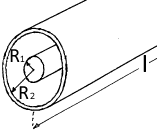
\includegraphics[width=4cm]{./pics/e-c-koaxialkabel.png}}
\parbox[t]{4.5cm}{\textbf{Doppelleitung} \\ \vspace{.2cm} \\
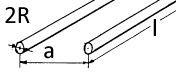
\includegraphics[width=4cm]{./pics/e-c-paralleldraht.png}}

\subsubsection{Plattenkondensator mit mehreren Dielektrika}
Grunds�tzlich kann gerechnet werden wie mit parallelen oder seriellen
Kondensatoren! Beispiel mit Luft und Dielektrika $\varepsilon_r$:
\\
\begin{tabular}{ll}
 Kapazit�t: &
$
\left.
\begin{aligned}
C_1 &= \frac{\varepsilon A}{d} = \frac{\varepsilon_0 A}{d-d_1} \\
C_2 &= \frac{\varepsilon A}{d} = \frac{\varepsilon_0 \varepsilon_r A}{d_1} 
\end{aligned}
\right\}
\quad C= \frac{C_1C_2}{C_1+C_2}
$ \\

Gespeicherte Energie: & 
$ W = \frac{1}{2}\cdot C \cdot U^2$
\end{tabular}
\parbox{6.5cm}{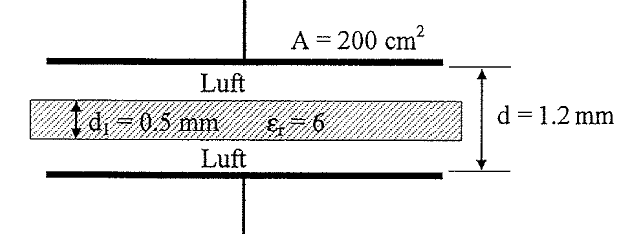
\includegraphics[width=6cm]{./pics/kond2dielekt.png}} \\

  
\subsection{Polarisation und Dielektrika}
\begin{tabular}{ll}
Im Homogenen Feld:&
$\frac{E_1}{E_2}=\frac{\epsilon_2}{\epsilon_1} $\\
Plattenkondensatoren mit verschiedenen Dielektrizit�tskonstanten: &
$U = E_1 d_1 + E_2 d_2 = \frac{D}{\epsilon_1} d_1 + \frac{D}{\epsilon_2} d_2
\Rightarrow D = \frac{U}{\frac{d_1}{\epsilon_1} + \frac{d_2}{\epsilon_2}}
\Rightarrow E_1 = \frac{D}{\epsilon_1}$\\
\end{tabular}

\parbox[t]{8.7cm} {
  \subsubsection{Feldlinien an Grenzfl. versch. Dielektrika}
  \parbox{4.5cm}{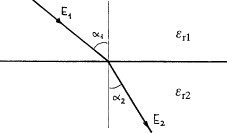
\includegraphics[width=4cm]{./pics/e-grenzflaechen-dielektrika}}
  \parbox{3.5cm}{
  $$ \frac{\tan(\alpha_1)}{\tan(\alpha_2)} = \frac{\varepsilon_{r1}}{\varepsilon_{r2}} $$ }
}
\parbox[t]{9.4cm}{
\subsubsection{Eigenschaften von Dielektrika}
  \tabcolsep0pt
  \begin{tabular}[t]{p{5.2cm} p{4.8cm}}
    homogen: $\varepsilon_r$ ist ortsunabh�ngig 
      & inhomogen: $\varepsilon_r$ ist ortsabh�ngig \\
    linear: $\varepsilon_r$ ist feldst�rkeunabh. 
      & nichtlinear: $\varepsilon_r$ ist feldst�rkeabh. \\ 
    isotrop: $\varepsilon_r$ ist richtungsunabh. 
      & anisotrop: $\varepsilon_r$ ist richtungsabh. 
  \end{tabular}
}

\subsection{Energie und Kraft im elektrostatischen Feld}
Im Kondensator gespeicherte Energie: $\qquad W = \frac{1}{2} \cdot C \cdot U^2 = \frac{1}{2} \cdot Q \cdot U = \frac{1}{2} \cdot \frac{Q^2}{C}$ \\
\parbox{5cm}{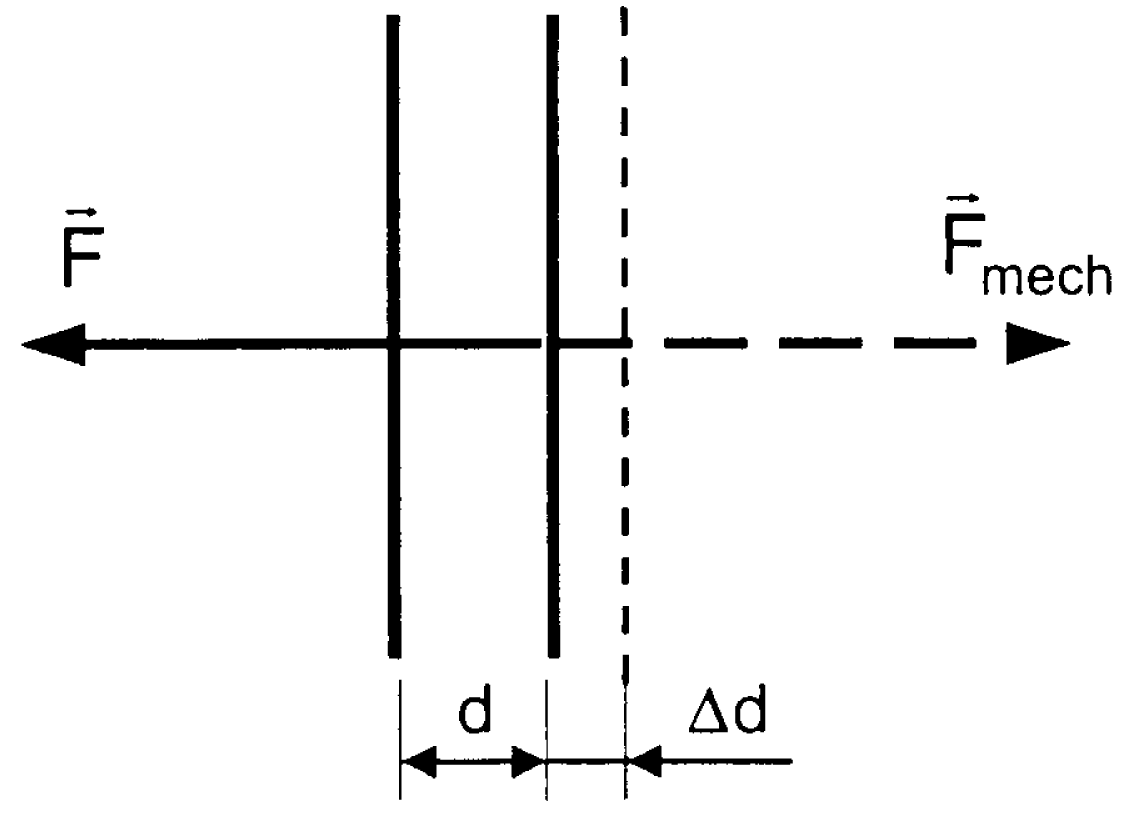
\includegraphics[width=4cm]{./pics/e-c-kraft}}
\parbox{13cm}{
  Grunds�tzlich versuchen sich die Feldlinien zu verk�rzen $\rightarrow$ Die Kraft auf die Grenzfl�chen ist so gerichtet, dass sie die Kapazit�t zu vergr�ssern sucht. \\ 
  Die Kraft berechnet sich mittels dem \textbf{Prinzip der virtuellen Verschiebung}. \\ \\
  $\qquad F = F_{mech} = \left| \frac{\Delta W}{\Delta d} \right| \qquad$ 
  $\Delta W = \frac{1}{2} \varepsilon \cdot E^2 \cdot A \cdot \Delta d \quad
  \Rightarrow \quad F = \frac{1}{2} \varepsilon \cdot E^2 \cdot A = \frac{1}{2}
  \varepsilon \cdot \frac{U^2}{d^2} \cdot A$ \\ $$ F =
  \frac{1}{2} \cdot U^2 \cdot \frac{\Delta C}{\Delta d}, \text{ (f�r U = const.)} \qquad \text{ oder } \qquad F = \frac{1}{2} \cdot Q^2 \cdot
  \frac{\mathrm d}{\Delta d} \left( \frac{1}{C} \right), \text{ (f�r Q =
  const.)}$$ \\
  Die Formel $F = \frac{1}{2}\varepsilon \cdot E^2 \cdot A$ gilt auch f�r
  Kondensatoren mit mehreren Dielektrika. Dazu wird einfach ein bekanntes
  $\varepsilon$ mit dem zugeh�rigen $E$ verwendet.}
  
  